
%3. Study of variance between models and data.  The optimized models part of this section is predicated on result 1b (so that optimization results can be believed).  You already have the poster for this.
%I think this captures most of your results in three themes.  Other results which are really methods, like parallel rheobase search, can stay in the methods, and you will get credit for them there.

\section{Published Models vs Optimized Models}
\label{sec:optimizing-published-models}
Neural models and real neurons may have divergent features.
Ideally, we would identify such features and modify the parameters (or form) of the models to eliminate this divergence.
This divergence may arise for two reasons: \emph{A} the model class was not flexible enough to simultaneously satisfy all of the constraints associated with those features, or \emph{B}: the model was incorrectly fitted to constraints that are inherently conflicting, due to issues in the underlying experimental data (see results for NeuroElectro data in previous sections).

In the absence of complete knowledge about the sources of model/experiment divergence for a given model, it is unknown which features should be used to fix the problem.
Modifying parameters to bring some features into alignment with experimental data may cause other features to fall out of alignment.
Ideally, we would identify that subset of features which, when handed to the optimizer, would produce a model which satisfies not only that feature subset, but all other features as well. 

I presented some features of membrane potential waveforms back in Section  \ref{sec:data-sources}.
Here I conducted a multivariate analysis analyzing hundreds of such features, asking which were useful for optimizing published neuron models to better reflect experimental data.
This high dimensional feature space is then summarized by a lower-dimensional subspace of key features on which optimized models differ from their pre-optimized published counterparts, as well as from experimental data.

%\begin{figure}
%    \centering
%    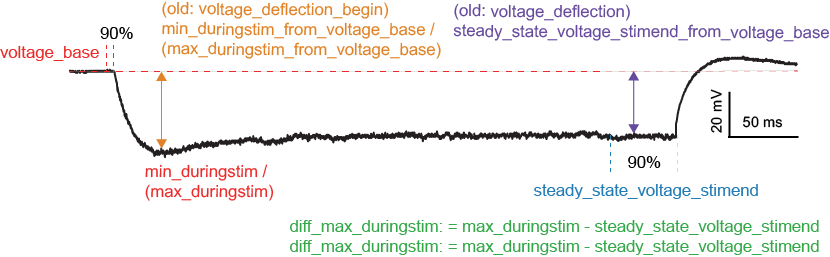
\includegraphics{figures/voltage_features.png}
%    \caption{Caption}
%    \label{fig:voltage_figures}
%\end{figure}
%\begin{figure}
%    \centering
%    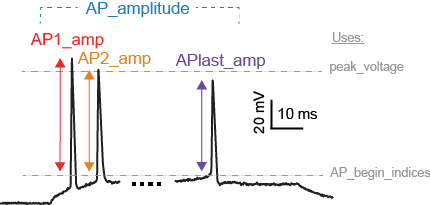
\includegraphics{figures/AP_Amplitude.png}
%    \caption{Caption}
%    \label{fig:features_example}
%\end{figure}

%\begin{figure}
%    \centering
%    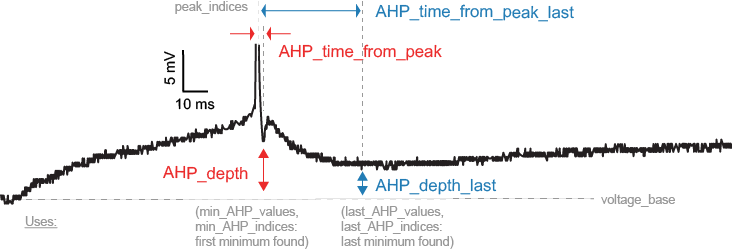
\includegraphics{figures/AHP.png}
%    \caption{After hyperpolarisation potential }
%    \label{fig:features_example_ahp}
%\end{figure}


%\begin{figure}
%    \centering
%    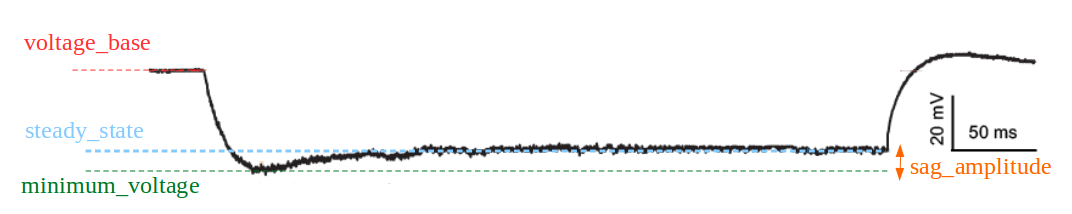
\includegraphics{figures/sag_amplitude}
%    \caption{Caption}
%    \label{fig:sag_amplitude}
%\end{figure}

\subsection{Models and Features} 
In order to conduct this analysis I used $972$ neuron models found in NeuroML-DB \citep{birgiolas2016rapid} and $448$ experiments on cortical neurons \emph{in vitro} from \cite{gouwens2018systematic} (example in Fig. \ref{fig:adaptionm}) and \cite{markram2006blue} (example in Fig. \ref{fig:bbp_trace_adaption_late_spike}).
%$1276$ samples. This did not include some blue brain cells. After data cleaning %many data points were dropped.  $244$
%$1420$
Although missing data imputation was used successfully to fill out the dataset, handling features that could not be fully imputed based on the available waveforms, about half of all initial models and experiments were nonetheless excluded from a final analysis, because they did not all capable of meeting inclusion criteria.
These include straightforward rules such as ``does this neuron exhibit spikes?", but also requirements about which stimuli were tested, and whether these were appropriate for computing the features that I used. 
Ultimately, 47 features were used for the subsequent analysis (out of a total of 466 from the initial list that are technically computable in some scenarios; see the Appendix for the full list).

%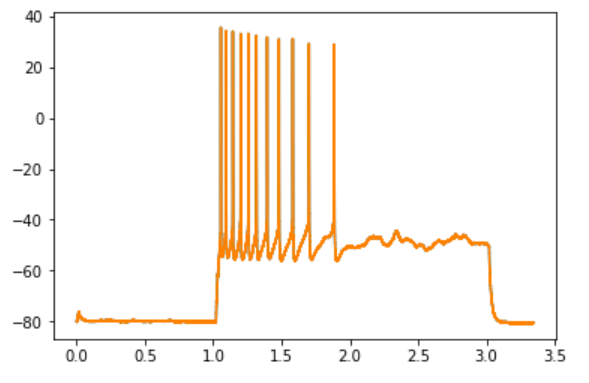
\includegraphics[]{chapters/app_tex/Allen_rush}
\begin{figure}
    \begin{center}
    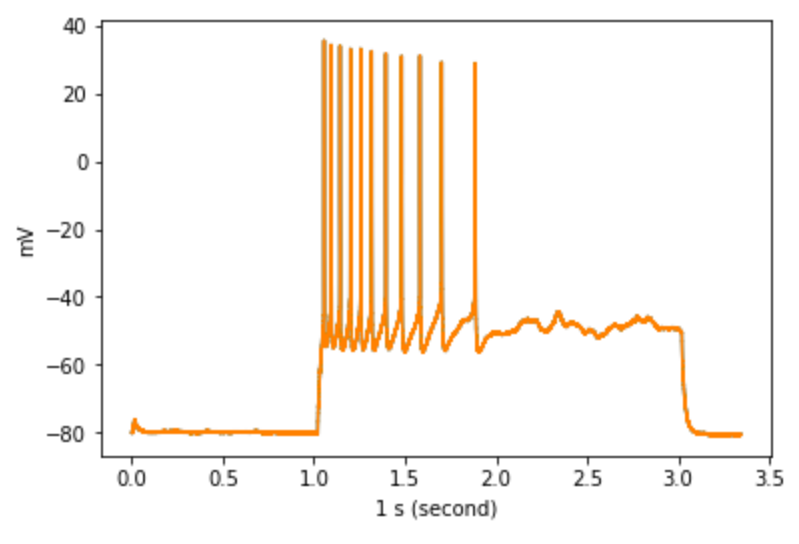
\includegraphics[width=0.6\linewidth]{figures/multi_spiking_large_allen}
    \caption[Example From Cell Types Database]{\textbf{Example data from the Allen Cell Types database}.
    Response of a real cortical cell to a supra-threshold stimulus in the Allen Brain Institute cell types data base \citep{gouwens2018systematic}.}
    \label{fig:adaptionm}
    \end{center}
\end{figure}    

\begin{figure}  
    \begin{center}
    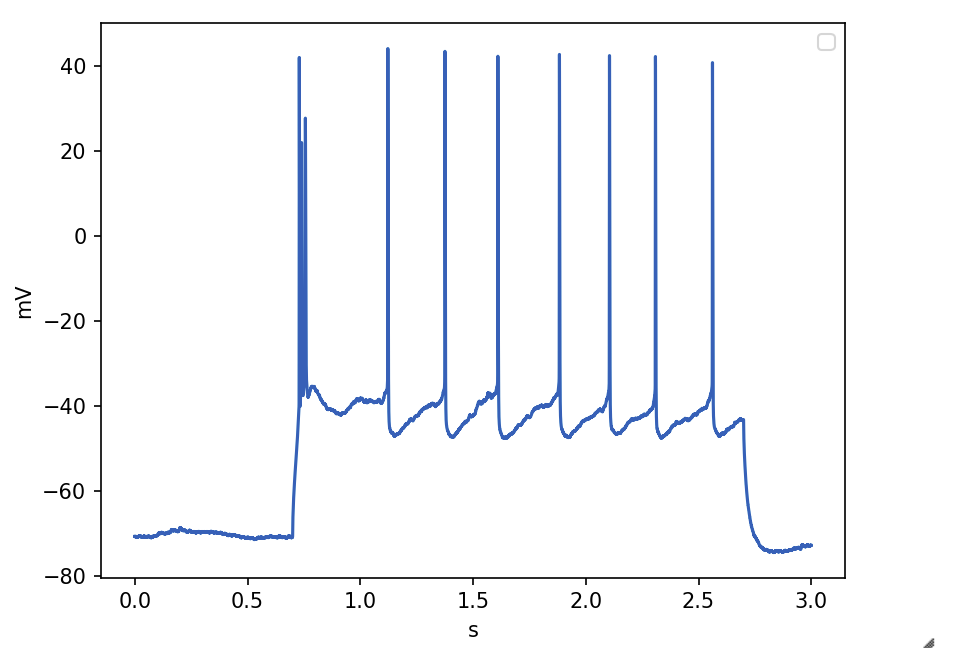
\includegraphics[width=0.6\linewidth]{figures/multi_spiking_large_bbp}
    \caption[Example From BBP]{\textbf{Example Data From the Allen Cell Types database}.
    Response of a real cortical cell to a supra-threshold stimulus in the Blue Brain Microcircuit Portal \citep{toledo}.}
    \label{fig:bbp_trace_adaption_late_spike}
    \end{center}
\end{figure}    

I applied feature extraction to the raw data from these experiments, using 3 approaches, which I adapted to NeuronUnit: (1) EFEL, developed by the Human Brain Project and described in section \ref{sec:efel}, (2) the Allen Institute SDK, developed as a companion to the Cell Types Database (but not exclusively so) and (3) \cite{druckmann2013hierarchical}, a general-purpose set of features for spike pattern analysis, as previously implemented for NeuronUnit in \cite{birgiolas2019towards}.
A common patterns was to apply somatic current injection at fixed multiples of rheobase, and extract features from the resulting spike patterns (Table \ref{table:three-step-stim}).

\begin{table}
\begin{center}
\begin{tabular}{|c|c|c|}
\toprule
Injection 1 & Injection 2 & Injection 3 \\
 \midrule
 $1.0 \times$ Rheobase current & $1.5 \times$ Rheobase current & $3.0 \times$ Rheobase current\\
\bottomrule
\end{tabular}
\caption[Three Step Stimulus Protocol]{Under the so-called three-step protocol, the rheobase current is first determined uniquely for each model or experiment, and features extracted from the response to this stimulus.
Then mutiples of rheobase ($\times 1.5$ and $\times 3.0$) are provided as stimuli, producing additional features that can be extracted using the library provided by \cite{EFEL}.
In the real experiments, similar protocols had been run (but using additive increments rather than multiples of rheobase).
I used interpolation to identify which of these additive increments to use as a proxy for the multiples of rheobase required to extract the current features.}
\label{table:three-step-stim}
\end{center}
\end{table}

\subsection{Identification of Salient Features}
In order to identify the electrophysiological measurements or ``features" that characterized variance in the models and the experimental data, as well as their differences, I performed Sparse Principle Component Analysis (Sparse PCA) \citep{zou2006sparse} on the ensemble.
Sparse PCA, unlike conventional PCA, yields readily interpretable components, each of which includes only a handful of features, rather than an indecipherable mix of all possible features. 
A low-dimensional embedding of models and data can then be obtained by re-plotting their features along the principal axes suggested by these components.
Sparse PCA yields an interpretable list of features, that build the principle components.

The non-zero loadings of Principle Component 1 are shown in Table \ref{table:spca-component1}.
This principal component did not distinguish between models and experiments, instead capturing a source of variance that was common to both of them.
By contrast, the second Principal Component discriminated models and experiments, indicating that it had captured some systematic difference between most published models and the experimental data for similar (but not necessarily the same) neurons.
It's non-zero loadings are shown in Table \ref{table:spca-component2}.
Models and experiments shared the same breadth of variability across the first principal component, with only slightly more variance in the experiments than in the data.
Allen Cell Types Database experiments exhibited the greatest variability out of all models and experiments (Figure \ref{fig:pca_data_points}).
Altogether, these two principal components were sufficient to partition models and data into three separate clusters (right panel in Figure \label{fig:pca_data_points}).
The full set of PCs are shown in Figure \ref{fig:spca-heatmap}.
Perhaps surprisingly, models clustered tightly and varied less than experimental data--one subset of Allen Cell Types database experiments even formed their own cluster--suggesting that perhaps past modeling efforts have been insufficiently bold in accounting for the diversity of cortical neuron types.

\begin{figure}    
    \begin{center}
    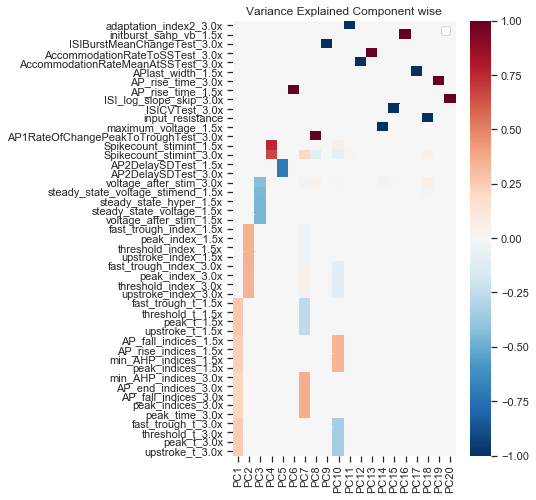
\includegraphics[scale=0.75]{figures/cortical_model_data_agreement_54_1.png}
    \caption[Sparse PCA Components]{\textbf{Sparse PCA Components}. Sparse PCA was applied to the collection of features extracted from models and data features.
    Component loadings from each feature were examined.
    Features are organized hierarchically, such that features with similar PC loadings are near each other.}
%fast_trough_indexes : numpy array of indexes at the start of the trough (i.e. end of the spike)
%adp_indexes : numpy array of adp indexes (np.nan if there was no ADP in that ISI
%slow_trough_indexes : numpy array of indexes at the minimum of the slow phase of the trough
    \end{center}
    \label{fig:spca-heatmap}
\end{figure}    

\begin{table}
\resizebox{\textwidth}{!}{
\begin{tabular}{|l|l|l|l|}
\toprule
Feature Name & Feature Description & Extraction Library &  Stimulus Strength \\
 upstroke-t & The time of upstrokes, this is the below $V_{T}$ first upward phase of AP & Allen & $1.5 \times$ Rheobase\\
 peak-t & Time(s) maximum $V_{M}$ occurs & Allen & $1.5 \times$ Rheobase \\
threshold-t & Time(s) $V_{T}$ is surpassed & Allen & $1.5 \times$ Rheobase \\
fast-trough-t & the times when when begginings of troughs were detected & Allen & $1.5 \times$ Rheobase \\ 
fast-trough-t & Same as above but at $3 \times$ Rheobase & Allen & $3.0 \times$ Rheobase \\
upstroke-t & Same as above but at $3 \times$ Rheobase & Allen & $3.0 \times$ Rheobase \\ 
peak-t & Same as above but at $3 \times$ Rheobase &Allen & $3.0 \times$ Rheobase \\ 
threshold-t & Same as above but at $3 \times$ Rheobase & Allen & $3.0 \times$ Rheobase \\ 
peak-indices & Indexs into array where peak voltages occur & EFEL & $1.5 \times$ Rheobase \\
min-AHP-indices & Indexs into array where minimum After Hyperpolarisation occur & EFEL & $1.5 \times$ Rheobase \\
\bottomrule
\end{tabular}
}
\caption[Features of First Principal Component in Sparse PCA]{
I identified the features associated with principal component 1 in the sparse PCA decomposition shown in Figure \ref{fig:spca-heatmap}.
These features explained $\frac{1}{3}$ of all of the variance (across models and data together), and were mainly associated with the timing of spikes and spike-associated events.
Notably, this principal component was not useful for separate models from experimental data.}
\label{table:spca-component1}
\end{table}

\begin{table}
\resizebox{\textwidth}{!}{
\begin{tabular}{|l|l|l|l|}
\toprule
Feature Name & Feature Description & Extraction Library  & Stimulus Strength \\
fast-trough-index & Index into array when begging of trough occurs & Allen & $1.5 \times$ Rheobase\\
peak-index-1.5x & Index into array when peaks occurs & Allen & $1.5 \times$ Rheobase \\
upstroke-index-1.5x & index into array of detection of first upward phase of AP & Allen & $1.5 \times$ Rheobase \\
threshold-index-1.5x & Description & Allen & $1.5 \times$ Rheobase \\ 
fast-trough-time & The time when a trough is commenced & Allen & $1.5 \times$ Rheobase \\
fast-trough-index & Indexs into array when the start of a trough is entered & Allen & $3.0 \times$ Rheobase \\ 
peak-index & indexs into array when voltage peak(s) occur & Allen & $3.0 \times$ Rheobase \\
upstroke-index & Index into array when first upward phase of a spike commences & Allen & $3.0 \times$ Rheobase \\ 
threshold-index & Index into array when threshold(s) are surpassed & Allen & $3.0 \times$ Rheobase \\
\bottomrule
\end{tabular}}
\caption[Features of Second Principal Component in Sparse PCA]{
The second principal component from the sparse PCA of Figure \ref{fig:spca-heatmap} contained features which describe spike shape.
Here, ``index" describes the location in the array of the extracted spike where an event occurs, thus it is relative to the timing of the spike itself, not to the timing of the stimulus.
These features contributed to the separation of models from experimental data.}
\label{table:spca-component2}
\end{table}

%Adaptation index 1 and adaptation 2 are the same but adaptation 2 evaluates for when there are skipped peaks. A skipped peak is when a spike or a spiklet does not surpass the nominated threshold for spike detection. 

%The parameter \myid{spike skipf} is the fraction of skipped peaks, $k$ is the minimum of \myid{spike skipf} times $N$ and \myid{max spike skip}.

% FAIL "Minimum 4 spike needed for feature [adaptation\_index]." \- \\
%The adaptation index is defined as "the Normalized average difference of two consecutive ISIs". "The adaptation index is zero for a constant firing rate and bigger than zero for a decreasing firing rate \citep{EFEL}"

  %All peaks in the time interval of \myid{stim start}$-$\myid{offset} and \myid{stim end}$+$\myid{offset} are regarded, \myid{offset} defaults to zero.
  
%pt$_0, \ldots, $pt$_{n-1} =$ peak\_time \\
%  pt$'_0$, \ldots, pt$'_{m-1}$  = $\{$ pt$_i$ | pt$_i \ge$ stim\_start $-$ offset AND pt$_i \le$ stim\_end $+$ offset $\}$ \\
%  $k = \min \{$ spike\_skipf $\cdot m$, max\_spike\_skip$\}$ \\
%  pt$''_0$, \ldots, pt$''_{l-1}$ = (pt$'_k$, \ldots, pt$'_m$) \\
%  IF $l$ < 4 THEN \+ \\
%    FAIL "Minimum 4 spike needed for feature [adaptation\_index]." \- \\
%  ENDIF \\
%  isi$_0$, \ldots, isi$_{j-1} =$ pt$''_1 -$ pt$''_0$, \ldots, pt$''_{l-1} -$ pt$''_{l-2}$ \\
%  sub$_0$, \ldots, sub$_{i-1} =$ isi$_1 -$ isi$_0$, \ldots, isi$_{j-1} -$ isi$_{j-2}$ \\
%  sum$_0$, \ldots, sum$_{i-1} =$ isi$_1 +$ isi$_0$, \ldots, isi$_{j-1} +$ isi$_{j-2}$ \\
%  APPEND $\frac{1}{i-1} \sum_{n=0}^{i-1} \frac{\mathrm{sub}_n}{\mathrm{sum}_n}$ TO adaptation\_index}
 % All peaks in the time interval of \myid{stim start}$-$\myid{offset} and \myid{stim end}$+$\myid{offset} are regarded, \myid{offset} defaults to zero.
%The adaptation index is zero for a constant firing rate and bigger than zero for a decreasing firing rate:
  
%Adaptation index 2  {Normalized average difference of two consecutive ISIs}

% The parameter \myid{spike skipf} is the fraction of skipped peaks, $k$ is the minimum of \myid{spike skipf} times $N$ and \myid{max spike skip}.

%\url{https://github.com/BlueBrain/eFEL/blob/master/docs/source/tex/efeatures.tex#L382}

Of the 48 of features considered, the features described in the table above make up the first two prinicipal components of sparse PCA decomposition, and are responsible for $\sim 50\%$ of the overall variance (left panel in Fig. \label{fig:pca_data_points}) in the ensemble of models and data.
Interestingly these features mostly belong to the Allen SDK feature extraction set, with two exceptions: \emph{peak-indices-1.5x}  and \emph{min-AHP-indices-1.5-times} which belong to EFEL.
This suggests that the Allen SDK might be nearly sufficient for both characterizing and discriminating between existing models and data.

\begin{figure}    
\begin{center} 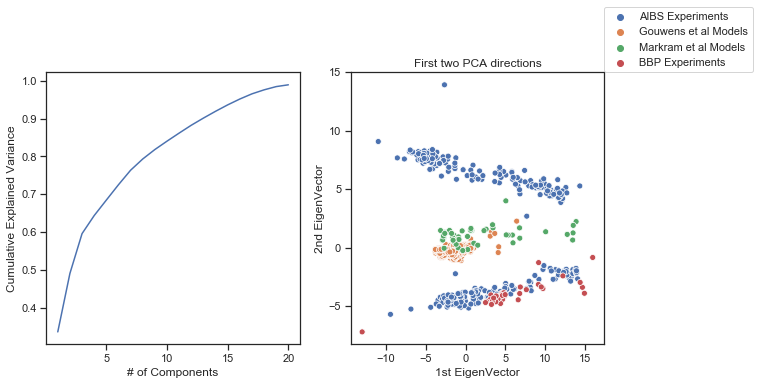
\includegraphics[width=1.0\linewidth]{figures/cortical_model_data_agreement_52_1}
\label{fig:}
\end{center}
\caption[Sparse PCA Clusters and Variance Explained]{Left panel: Sparse PCA could explain $\sim95\%$ of the variance in the ensemble of model and experimental data features using $\sim15$ components, but the first two were sufficient to explain $\sim50\%$ of the variance.
Right panel: A cluster analysis revealed revealed three major clusters of feature values.
Models and experimental data could be distinguished by PC 2.
Individual dots refer to experiments from the Allen Institute Cell Types database (blue), model published by the Allen Institute (orange), experiments published by the Blue Brain Project (red), and models published by the Blue Brain Project (orange).
}
%In figures (\ref{fig:TSNE}, and 
%\ref{fig:pca_cluster}) shown below, I introduce some spurious results. Those should not be confused with results in this figure, which I am confident about}
\label{fig:pca_data_points}
\end{figure}    


\begin{comment}
\subsubsection{Proto-type of Secondary Validation Pathway}
Neuronunits ability to do evaluate a $\chi^{2}$ hypothesis test constitutes a valuable model validation pathway, however, it is desirable to have several indipendant model validation approaches. 
\begin{figure}    
\begin{center} 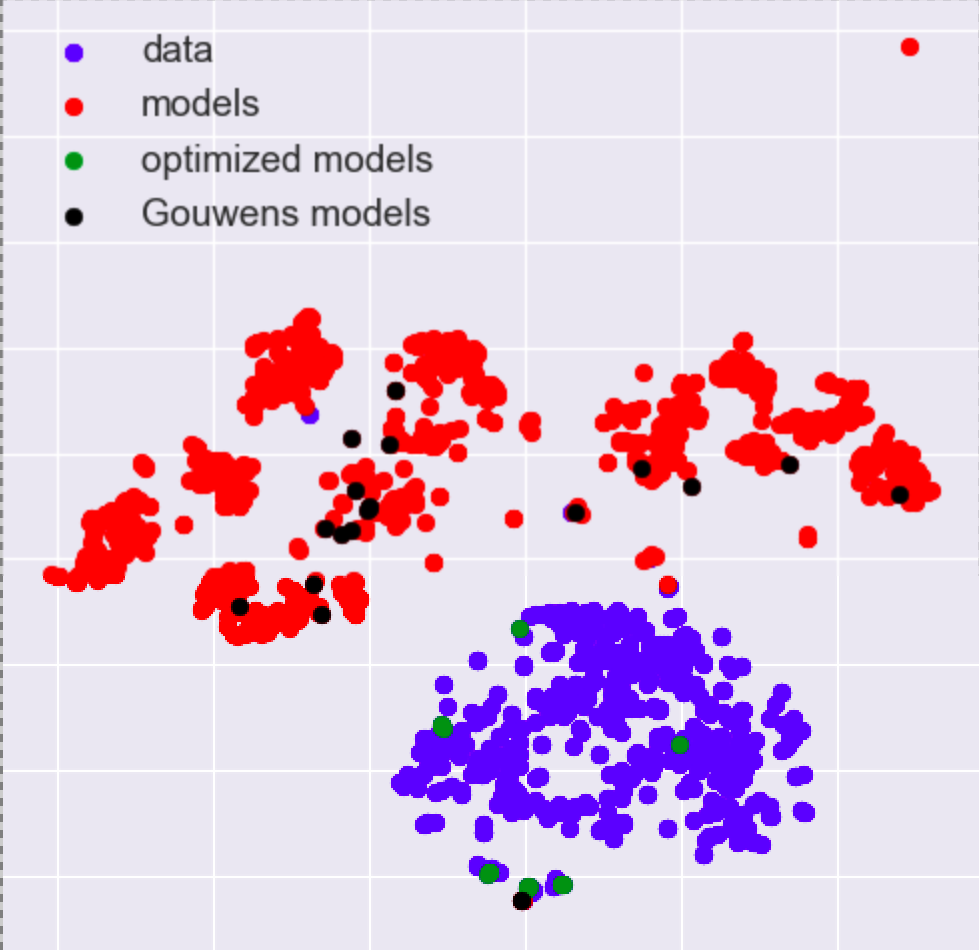
\includegraphics[width=0.5\linewidth]{figures/optimized_model_fit_onto_big_distribution.png}
\label{fig:TSNE}
\end{center}
\caption[A TSNE Low Spatial Embedding Optimized Models]{A TSNE spatial embedding. The data point positions in this plot were later identified to be spurious, however the plot should not be interpreted as a finding, but as a prototype of a valuable validation pathway.}

%showing how optimized models, fair relative to other published models. Looking at this plot, the first interpretation is one of great optimism. Other interpretations are possible.}
\label{fig:tsne_opt_model_points}
\end{figure}    

\begin{figure}    
\begin{center} 
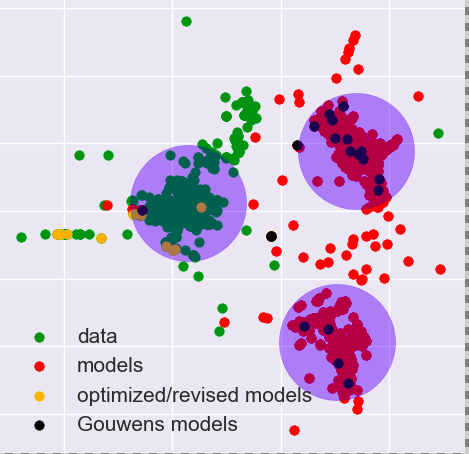
\includegraphics[width=0.5\linewidth]{figures/data_experiment_fits.png}
\end{center}
\caption[PCA with Cluster Centers]{ Similar Dimensionality reduction to above, but instead PCA is used instead of TSNE, and cluster centers drawn. The purpose of this plot is to introduce the prototype of a validation pathway, although specific data points shown here are spurious.}
\label{fig:pca_cluster}
\end{figure}    

In figures (\ref{fig:tsne_opt_model_points} and \ref{fig:pca_cluster}). I have projected pre-optimized models into the same low dimensional embedding, given by some dimensionality reduction algorithms. The advantage of such plots is that in theory they provide a separate and indipendent means of validating models outside of the neuronunit-Zscore frame work. Additionally they provide a means to e valuate generality of model fits, as the models here where only optimized against 8 different Neuroelectro tests (of at or below threshold behaviors), in this new context, those same cells are now being compared against 48 different spike-train-shape features.

Inspecting In figures (\ref{fig:tsne_opt_model_points} and \ref{fig:pca_cluster}). It looks as if optimized (Izhikevich) models, are better fits for experimental data, than many pre-published models, since the optimized models (yellow) are clustered with the experiments (green). There are some important caveats that make drawing strong optimistic conclusions hard. The first caveat is that at this point, about 50\% of rows, had many absent features that where filled with $0s$, the rest had significantly normal values in the missing features. This artifact artificially boosted variance in several features, that realistically lacked variance. Once the zeros where identified and imputed, other real sources of variance in the data were much more highly weighted in their contribution to PCA transformation. With other variance sources now weighted more highly, the optimized cells where repositioned more distant from the experimental cluster.

As I have discussed, some of the earlier work in this area was later, in-validated, once I had identified some artificial sources of variance.
\end{comment}


%Figure \label{fig:pca_data_points}, shows the a rigorous low dimensional embedding of the 48 dimension feature space. Earlier I produced figures: (\ref{fig:tsne_opt_model_points} and \ref{fig:pca_cluster}). The overall structure of the three different plots is inconsistent to a degree which is greater than what can be attributed to in differences of dimensionality reduction algorithm. In the final rigorous plot (\label{fig:pca_data_points}) it is experimental data that falls into two clusters, and models fall into a single central cluster. In the earlier less rigorous plots models fall into two clusters and experiments are united in one central cluster.


% In the low dimensional embedding, could  optimized reduced models where plotted

% Unfortunately there were some confounding factors.


A small majority of features identified by sparse PCA are derived from the $1.5 \times$ rheobase stimulus, slightly fewer are from the $3.0\times$ rheobase stimulus.
This may be because spike time and spike count variability in the most sensitive (highest slope) part of the FI curve, slightly above rheobase, is greater than under the highest current injections, where the neuron is much close to responding as quickly as possible (i.e. near its absolute refractory period).

\subsection{What Distinguishes Published Models from Experimental Data?}
Disagreement between models and real neurons may reflect limitations of model design and can be investigated by probing the features identified by a classifiers trained to distinguish these two populations. 
Figure \ref{fig:from-poster_disagree} shows the distributions of two features for models (red) and for experimental data (blue).
Rather than the distributions being separable, the major observation is that the distribution of these features across published models is simply much narrower.
The diversity of feature values in real neurons is simply not being adequately captured by published models.
%\cite{wang2019sag}

\begin{figure}
    \centering
    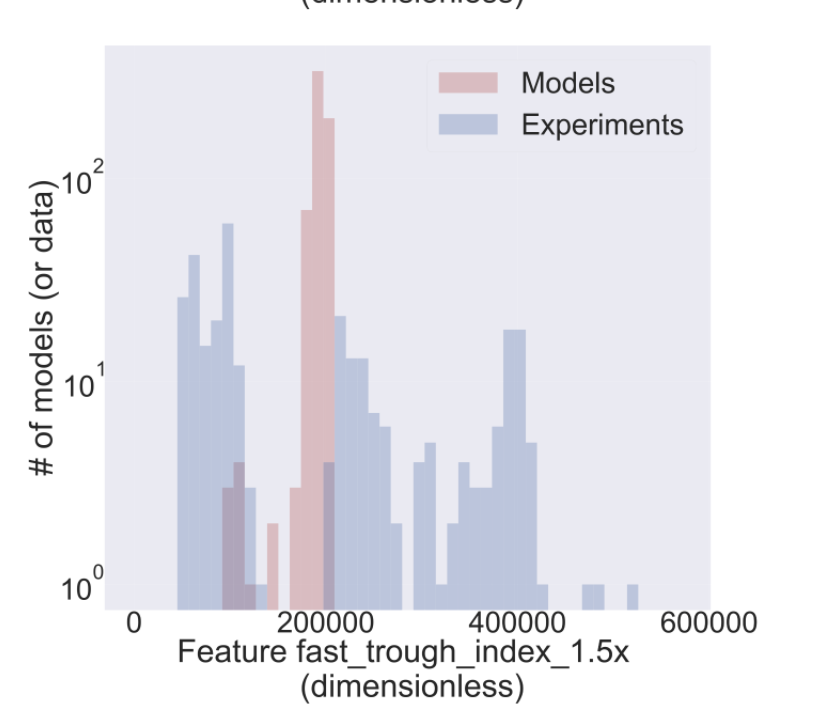
\includegraphics[scale=0.5]{figures/fast_trough}
    \caption[Comparison of Model and Experiment Feature Distributions (A)]{The variance of single features across biological neurons (blue) is much greater than that observed in published models.
    The feature shown here (fast-trough-index) reflects the latencies of the post-spike trough relative to its peak.
    Biological neurons clearly exhibit a wide range of such latencies, where as models exhibit a narrow range possibly limited by their underlying dynamics.
    }
    \label{fig:from-poster-disagree}
\end{figure}

\begin{figure}
    \centering
    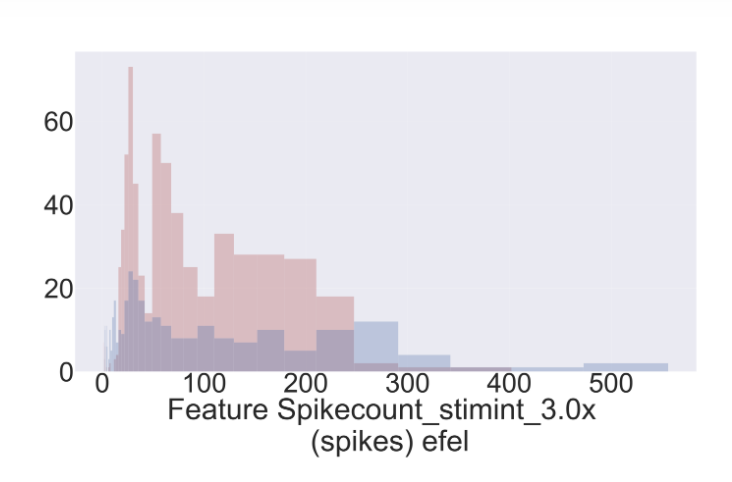
\includegraphics[scale=0.75]{figures/spike_count_at_3rheobase.png}
    \caption[Comparison of Model and Experiment Feature Distributions (A)]{Unlike Figure \ref{fig:from-poster-disagree}, some features showed comparably wide distributions in model and biological neurons.
    The distribution of spike counts is similarly skewed in both cases.
    This suggests that, in contrast to spike shapes, reduced models are able to reflect the diversity of overall firing rate statistics seen in biology.
    %The sparse PCA graph is very abstract, it's important to understand that much variance found by the sparse PCA algorithm originates from differences between model distributions and experiment distributions Simple stacked histograms of data are able to show such differences. By "Fast" in fast trough indexs, all that is meant is the beginning time of troughs occurrence, this would contrast with the "slow" or ending time of the spikes. This is arguably a bad naming scheme.
    }
    \label{fig:from_poster_disagree}
\end{figure}
%\begin{figure}
%    \centering
%    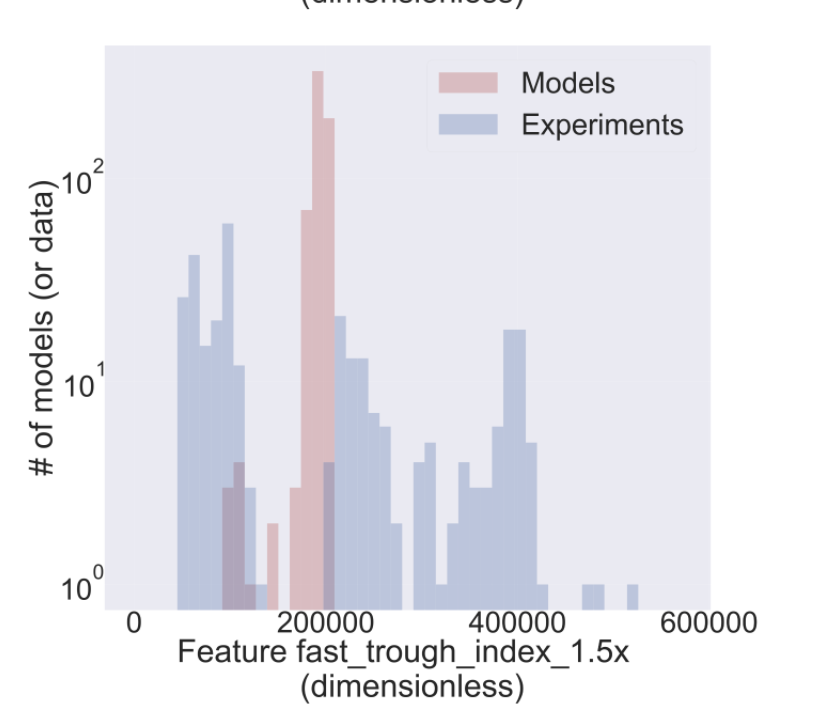
\includegraphics[scale=0.75]{figures/fast_trough}
%    \caption[Features that agree. SpikeCount]{
%    Not all features disagreed. Example of Agreement: spike counts in models and experiments. The sparse PCA graph is very abstract, it's important to understand that much variance found by the sparse PCA algorithm originates from differences between model distributions and experiment distributions Simple stacked histograms of data are able to show such differences. By "Fast" in fast trough indexs, all that is meant is the beginning time of troughs occurrence, this would contrast with the "slow" or ending time of the spikes. This is arguably a bad naming scheme.
%    \url{https://allensdk.readthedocs.io/en/latest/allensdk.ephys.ephys_features.html}
%    }
%    \label{fig:from_poster_disagree}
%\end{figure}


%\begin{comment}
%\begin{itemize}
%    \item upstroke\_t\_1.5x allen feature
%    \item  peak\_t\_1.5x allen feature
%    \item threshold\_t\_1.5x allen feature
%    \item fast\_trough\_t\_1.5x allen feature
%    \item fast\_trough\_t\_3.0x allen feature
%    \item upstroke\_t\_3.0x allen feature
%    \item peak\_t\_3.0x allen feature
%    \item threshold\_t\_3.0x allen feature
%    \item peak\_indices\_1.5x efel feature
%    \item min\_AHP\_indices\_1.5x efel feature
%\end{itemize}
%\end{comment}


%\begin{itemize}
%    \item fast\_trough\_index\_1.5x allen feature
%    \item fast\_trough\_index\_3.0x allen feature
%    \item threshold\_index\_1.5x allen feature
%    \item peak\_index\_1.5x allen feature
%    \item upstroke\_index\_1.5x allen feature
%    \item peak\_index\_3.0x allen feature
%    \item upstroke\_index\_3.0x allen feature
%    \item threshold\_index\_3.0x allen feature
%\end{itemize}

%After identifying specific sources of model and experiment divergence, it is %now possible in theory to start fitting models which seek to resolve specific %types of disagreement.
%However, as alluded to in the introduction, it was found that were two other %important factors. 

%Model repurposing is common and it is done on a network scale \cite{traub} and an individual cell scale.
%Experimental evidence is starting to reveal that model re-purposing of pyramidal neurons might not be a good idea.

%Scientific insight is well-served by the discovery and optimization of abstract models that can reproduce experimental findings. NeuroML (NeuroML.org), a model description language for neuroscience, facilitates reproducibility and exchange of such models by providing an implementation-agnostic model description in a modular format. NeuronUnit (neuronunit.scidash.org) evaluates model accuracy by subjecting models to experimental data-driven validation tests, a formalization of the scientific method. 


% After applying dimensionality reduction to this very high dimensional feature space, we show that the real (biological neurons) and simulated (model neurons) recordings are easiley and fully discriminated by eye or any reasonable classifier.  

% Are they still discernable?
%972 models, 448 experiments.


%Consequently, not a single model neuron produced physiological responses that could be confused with a biological neuron. Was this a defect of the model design (e.g. key mechanisms unaccounted for) or of model parameterization? We found that if we introduced models that were revised via optimization the revised models overlapped with the distribution of biological neurons, and were mostly classified as such. 
